\documentclass[10pt,handout]{beamer}\usepackage[]{graphicx}\usepackage[]{color}
% maxwidth is the original width if it is less than linewidth
% otherwise use linewidth (to make sure the graphics do not exceed the margin)
\makeatletter
\def\maxwidth{ %
  \ifdim\Gin@nat@width>\linewidth
    \linewidth
  \else
    \Gin@nat@width
  \fi
}
\makeatother

\definecolor{fgcolor}{rgb}{0.345, 0.345, 0.345}
\newcommand{\hlnum}[1]{\textcolor[rgb]{0.686,0.059,0.569}{#1}}%
\newcommand{\hlstr}[1]{\textcolor[rgb]{0.192,0.494,0.8}{#1}}%
\newcommand{\hlcom}[1]{\textcolor[rgb]{0.678,0.584,0.686}{\textit{#1}}}%
\newcommand{\hlopt}[1]{\textcolor[rgb]{0,0,0}{#1}}%
\newcommand{\hlstd}[1]{\textcolor[rgb]{0.345,0.345,0.345}{#1}}%
\newcommand{\hlkwa}[1]{\textcolor[rgb]{0.161,0.373,0.58}{\textbf{#1}}}%
\newcommand{\hlkwb}[1]{\textcolor[rgb]{0.69,0.353,0.396}{#1}}%
\newcommand{\hlkwc}[1]{\textcolor[rgb]{0.333,0.667,0.333}{#1}}%
\newcommand{\hlkwd}[1]{\textcolor[rgb]{0.737,0.353,0.396}{\textbf{#1}}}%
\let\hlipl\hlkwb

\usepackage{framed}
\makeatletter
\newenvironment{kframe}{%
 \def\at@end@of@kframe{}%
 \ifinner\ifhmode%
  \def\at@end@of@kframe{\end{minipage}}%
  \begin{minipage}{\columnwidth}%
 \fi\fi%
 \def\FrameCommand##1{\hskip\@totalleftmargin \hskip-\fboxsep
 \colorbox{shadecolor}{##1}\hskip-\fboxsep
     % There is no \\@totalrightmargin, so:
     \hskip-\linewidth \hskip-\@totalleftmargin \hskip\columnwidth}%
 \MakeFramed {\advance\hsize-\width
   \@totalleftmargin\z@ \linewidth\hsize
   \@setminipage}}%
 {\par\unskip\endMakeFramed%
 \at@end@of@kframe}
\makeatother

\definecolor{shadecolor}{rgb}{.97, .97, .97}
\definecolor{messagecolor}{rgb}{0, 0, 0}
\definecolor{warningcolor}{rgb}{1, 0, 1}
\definecolor{errorcolor}{rgb}{1, 0, 0}
\newenvironment{knitrout}{}{} % an empty environment to be redefined in TeX

\usepackage{alltt}


%\input{slides_header.tex}
\usepackage{graphicx}
\usepackage{hyperref, url}
\hypersetup{colorlinks,citecolor=myorange,filecolor=red,linkcolor=brown,urlcolor=blue}

\usepackage{longtable,booktabs}
\usepackage{amssymb,amsmath}
\usepackage{animate}
\usepackage{subfig}
\usepackage{tikz}
\usetikzlibrary{shapes.geometric, arrows,shapes.symbols,decorations.pathreplacing}
\tikzstyle{startstop} = [rectangle, rounded corners, minimum width=3cm, minimum height=1cm, draw=black, fill=pinkish,text width=3.5cm]
\tikzstyle{startstop2} = [rectangle, rounded corners, minimum width=3cm, minimum height=1cm, draw=black, fill=background,text width=4.5cm]
\tikzstyle{startstop3} = [rectangle, rounded corners, minimum width=3cm, minimum height=1cm, draw=black, fill=beige,text width=3.0cm]
\tikzstyle{startstop4} = [rectangle, rounded corners, minimum width=3cm, minimum height=1cm, draw=black, fill=pinkish,text width=4.5cm]
\tikzstyle{io} = [trapezium, trapezium left angle=70, trapezium right angle=110, minimum width=2cm, minimum height=1cm, text centered, draw=black, fill=blue!30,text width=1.5cm]
\tikzstyle{process} = [rectangle, minimum width=1cm, minimum height=1cm, text centered, draw=black, fill=orange!30,text width=2cm]
\tikzstyle{decision} = [diamond, minimum width=2cm, minimum height=1cm, text centered, draw=black, fill=green!30]
\tikzstyle{arrow} = [thick,->,>=stealth]
\tikzstyle{both} = [thick,<->,>=stealth, red]


% used for tree of stats tests in 001-introduction
\tikzstyle{startstopstats} = [rectangle, rounded corners, minimum width=2cm, minimum height=.5cm,text centered, draw=black, fill=red!30]
\tikzstyle{iostats} = [trapezium, trapezium left angle=70, trapezium right angle=110, minimum width=2cm, minimum height=.5cm, text centered, draw=black, fill=blue!30]
\tikzstyle{processstats} = [rectangle, minimum width=1.5cm, minimum height=.5cm, text centered, draw=black, fill=orange!30]
\tikzstyle{processbigstats} = [rectangle, minimum width=1.5cm, minimum height=.5cm, text centered, draw=black, fill=orange!30,text width=1.6cm]
\tikzstyle{decisionstats} = [rectangle, minimum width=1cm, minimum height=1cm, text centered, draw=black, fill=green!30,text width=1.6cm]
\tikzstyle{decisionbigstats} = [rectangle, minimum width=1cm, minimum height=1cm, text centered, draw=black, fill=yellow!30,text width=2cm]

\usepackage{pifont}% http://ctan.org/pkg/pifont
\newcommand{\cmark}{\ding{51}}%
\newcommand{\xmark}{\ding{55}}%

\usepackage{ulem} % for strikeout

\usepackage{xcolor}
\usepackage{color, colortbl}
\definecolor{lightgray}{RGB}{200,200,200}
\definecolor{palegray}{RGB}{221,221,221}
\definecolor{myblue}{RGB}{0,89,179}
\definecolor{myorange}{rgb}{0.776,0.357,0.157}
\definecolor{gray}{RGB}{110,110,110}
\definecolor{darkgray}{RGB}{100,100,100}
\definecolor{lightgray}{RGB}{200,200,200}
\definecolor{palegray}{RGB}{221,221,221}
\definecolor{turquoise}{RGB}{81,193,188}
\definecolor{tomato}{RGB}{255,136,136}
\definecolor{mandarina}{RGB}{229,169,25}
\definecolor{foreground}{RGB}{81,141,193}
\definecolor{background}{RGB}{246,244,240}
\definecolor{highlight}{RGB}{229,169,25}
\definecolor{lowlight}{RGB}{200,200,200}
\definecolor{beige}{RGB}{255,255,240}
\definecolor{pinkish}{RGB}{255,223,247}
\definecolor{darktangerine}{rgb}{1.0, 0.66, 0.07}
\definecolor{deepink}{RGB}{255,20,147}
%\usepackage{shadethm}
%\colorlet{shadecolor}{blue!15}
%\colorlet{shadecolor}{palegray}
%\setlength{\shadeboxrule}{.4pt}

%\newshadetheorem{thm}{Theorem}
%\newshadetheorem{defm}{Definition}
%\newshadetheorem{exm}{Exercise}
%\newshadetheorem{remarkm}{Remark}
%\definecolor{shadethmcolor}{HTML}{EDF8FF}
%\definecolor{shadethmcolor}{RGB}{221,221,221}
%\definecolor{shaderulecolor}{HTML}{45CFFF}
%\definecolor{shaderulecolor}{RGB}{0,89,179}
%\setlength{\shadeboxrule}{.4pt}



\usepackage{epsfig}

\newcommand{\code}[1]{\texttt{#1}}
\newcommand{\blue}[1]{\textcolor{blue}{#1}}
\newcommand{\red}[1]{\textcolor{red}{#1}}

\usepackage{comment}

\makeatletter

\def \iqsssectiontitleheader {}

\newcommand{\iqsssectiontitle}[1]{
	\def \iqsssectiontitleheader{#1}
}

\@ifundefined{insertmainframenumber}
{%
	% \insertmainframenumber not defined
	\newcommand{\insertmainframenumber}{\inserttotalframenumber}
}
{%
	% \insertmainframenumber already defined
}%


\AtBeginSection[]{
	\title{\insertsectionhead}
	{
		%\definecolor{white}{RGB}{140,193,250}
		%\definecolor{white}{RGB}{200,200,200}
		%\definecolor{white}{RGB}{242,244,247}
		\definecolor{white}{RGB}{0,89,179}
		%\definecolor{iqss@orange}{rgb}{1,1,1}
		\ifnum \insertmainframenumber > \insertframenumber
		%\setbeamercolor{background canvas}{bg=myblue}
		%\setbeamercolor{normal text}{fg=black,bg=white}
		%\setbeamercolor{frametitle}{fg=red}
		%\setbeamercolor{section in toc}{fg=myblue, bg=white}
		%\setbeamercolor{subsection in toc}{fg=myblue, bg=white}
		\frame{
			\frametitle{\iqsssectiontitleheader}
			\tableofcontents[currentsection]
		}
		\else
		\frame{
			\frametitle{Backup Slides}
			\tableofcontents[sectionstyle=shaded/shaded,subsectionstyle=shaded/shaded/shaded]
		}
		\fi
	}
}
\makeatother
%\graphicspath{{/home/sahir/git_repositories/EPIB607/resources/assets/slides/figure/}}


\usepackage{fontspec}
%\setsansfont{Fira Sans}
%\setmonofont{Fira Mono}
%\setsansfont[ItalicFont={Fira Sans Light Italic},BoldFont={Fira Sans},BoldItalicFont={Fira Sans Italic}]{Fira Sans Light}
%\setmonofont[BoldFont={Fira Mono Medium}]{Fira Mono}

\def\installpath{/usr/local/share/texmf/fonts/opentype/libertinus/}
\setmainfont{LibertinusSerif}[
UprightFont    = *-Regular,
BoldFont       = *-Bold,
ItalicFont     = *-Italic,
BoldItalicFont = *-BoldItalic,
Ligatures      = TeX,
Extension      = .otf,
Path           = \installpath/
]

\setsansfont{LibertinusSerif}[
UprightFont    = *-Regular,
BoldFont       = *-Bold,
ItalicFont     = *-Italic,
BoldItalicFont = *-BoldItalic,
Ligatures      = TeX,
Extension      = .otf,
Path           = \installpath/
]


%\setmonofont{LibertinusSerif}[
%UprightFont    = *-Regular,
%BoldFont       = *-Bold,
%ItalicFont     = *-Italic,
%BoldItalicFont = *-BoldItalic,
%Ligatures      = TeX,
%Extension      = .otf,
%Path           = \installpath/
%]






\newcommand\Wider[2][3em]{%
	\makebox[\linewidth][c]{%
		\begin{minipage}{\dimexpr\textwidth+#1\relax}
			\raggedright#2
		\end{minipage}%
	}%
}


\newcommand {\framedgraphic}[1] {
	\begin{figure}
		\centering
		\includegraphics[width=\textwidth,height=0.9\textheight,keepaspectratio]{#1}
	\end{figure}
}


\newcommand {\framedgraphiccaption}[2] {
	\begin{figure}
		\centering
		\includegraphics[width=\textwidth,height=0.8\textheight,keepaspectratio]{#1}
		\caption{#2}
	\end{figure}
}




\setbeamercolor{itemize item}{fg=myblue}
\setbeamercolor{itemize subitem}{fg=myorange}
%\setbeamertemplate{itemize item}[square]
\setbeamertemplate{itemize item}[circle]
\setbeamertemplate{itemize subitem}[triangle]
\setbeamertemplate{blocks}[rounded][shadow=true]
\setbeamercolor{block body alerted}{bg=alerted text.fg!10}
\setbeamercolor{block title alerted}{bg=alerted text.fg!20}
\setbeamercolor{block body}{bg=structure!10}
\setbeamercolor{block title}{bg=structure!20}
\setbeamercolor{block body example}{bg=green!10}
\setbeamercolor{block title example}{bg=green!20}


\makeatletter
\newenvironment<>{proofs}[1][\proofname]{%
	\par
	\def\insertproofname{#1\@addpunct{.}}%
	\usebeamertemplate{proof begin}#2}
{\usebeamertemplate{proof end}}
\newenvironment<>{proofc}{%
	\setbeamertemplate{proof begin}{\begin{block}{}}
		\par
		\usebeamertemplate{proof begin}}
	{\usebeamertemplate{proof end}}
	\newenvironment<>{proofe}{%
		\par
		\pushQED{\qed}
		\setbeamertemplate{proof begin}{\begin{block}{}}
			\usebeamertemplate{proof begin}}
		{\popQED\usebeamertemplate{proof end}}
\makeatother


\makeatletter
\newenvironment<>{exams}[1][\proofname]{%
	\par
	\def\insertproofname{#1\@addpunct{.}}%
	\usebeamertemplate{example begin}#2}
{\usebeamertemplate{example end}}
\newenvironment<>{examc}{%
	\setbeamertemplate{exam begin}{\begin{block}{}}
		\par
		\usebeamertemplate{exam begin}}
	{\usebeamertemplate{exam end}}
	\newenvironment<>{exame}{%
		\par
		\pushQED{\qed}
		\setbeamertemplate{exam begin}{\begin{block}{}}
			\usebeamertemplate{exam begin}}
		{\popQED\usebeamertemplate{exam end}}
		\makeatother

%\definecolor{mycolor}{HTML}{F7F8E0}
%\declaretheorem[shaded={bgcolor=mandarina}]{theo}
%\declaretheorem[shaded={bgcolor=mycolor}]{propo}
%\declaretheorem[shaded={bgcolor=green!80!black!30}]{remark}

%\setbeamertemplate{navigation symbols}{\usebeamercolor[fg]{title in head/foot}\usebeamerfont{title in head/foot}\insertframenumber}


%\setbeamertemplate{footline}{}

\beamertemplatenavigationsymbolsempty % toggle off if you want navigation symbols at the bottom

\setbeamertemplate{footline}
{ \usebeamercolor[fg]{page number in head/foot}%
	\usebeamerfont{page number in head/foot}%
	\hspace{1em}\insertsectionhead%
	\hfill%
	\insertframenumber\,/\,\hyperlinkappendixstart{\insertmainframenumber}
	\ifnum \thepage = \insertframeendpage{\small .}\else{\phantom{\small .}}\fi
	\hspace{1em}
	\vskip2pt%
}

%\newtheorem{proposition}[theorem]{Proposition}
%\newtheorem{exercise}[theorem]{Exercise}
%\newtheorem{remark}[theorem]{Remark}


\usepackage{amsthm}
\usepackage{thmtools}

\setbeamertemplate{theorems}[ams style] 
%\setbeamertemplate{theorems}[numbered] 
%\setbeamertemplate{corollary}[numbered] 
\newtheorem{proposition}{Proposition}
\newtheorem{exercise}{Exercise}
\newtheorem{remark}{Remark}
\newtheorem{exam}{Example}
%\newtheorem{proof}{Proof}
%\newtheorem{corollaries}[theorem]{Corollary}
\newcommand*{\theorembreak}{\usebeamertemplate{theorem end}\framebreak\usebeamertemplate{theorem begin}}



\setlength{\emergencystretch}{3em} % prevent overfull lines
\providecommand{\tightlist}{%
	\setlength{\itemsep}{0pt}\setlength{\parskip}{0pt}}

\newcommand\AddButton{%
	\setbeamertemplate{background canvas}{%
		\begin{tikzpicture}[remember picture,overlay]
		\node[anchor=west] at ([yshift=5pt,xshift=0.1em]current page.south west)
		{\hyperlink{toc}{\beamergotobutton{back to TOC}}};
		\end{tikzpicture}%
	}%
}


\titlegraphic{\hfill
\includegraphics[height=1cm]{/home/sahir/git_repositories/EPIB607/slides/mcgill_logo.png}}




\graphicspath{{/home/sahir/git_repositories/EPIB607/slides/figure/}}

%\let\oldShaded\Shaded
%\let\endoldShaded\endShaded
%\renewenvironment{Shaded}{\footnotesize\oldShaded}{\endoldShaded}

\newcommand{\Var}{\operatorname{Var}}
\newcommand{\Expec}{\operatorname{E}}
\newcommand{\Prob}{\operatorname{P}}
\IfFileExists{upquote.sty}{\usepackage{upquote}}{}
\begin{document}



%\title{Introduction to Regression Trees}
%\author{Sahir Bhatnagar \inst{1}}
%\author[shortname]{Sahir Rai Bhatnagar, PhD Candidate (Biostatistics) }
%\institute[shortinst]{Department of Epidemiology, Biostatistics and Occupational Health}

\title{009 - Random Variables}
\author{EPIB 607}
\institute{
	Sahir Rai Bhatnagar\\
	Department of Epidemiology, Biostatistics, and Occupational Health\\
	McGill University\\
	
	\vspace{0.1 in}
	
	\texttt{sahir.bhatnagar@mcgill.ca}\\
	\texttt{\url{https://sahirbhatnagar.com/EPIB607/randomVariables.html}}
}

\date{slides compiled on \today}

\maketitle

\section{Random Variables}

\begin{frame}{Introduction}

	\begin{itemize}
					  \setlength{\itemsep}{10pt}
		\item  This central chapter addresses a fundamental concept, namely the laws governing the variance of a sum of 2, or (especially) $n$ random variables  -- and even more importantly -- the laws governing the variance of a difference of two random variables. 
		\item The latter is  central, not just to simple contrasts involving 2 sample means or proportions, but also in the much wider world of regression, since the variance (sampling variability) of any regression slope can be viewed as the variance of a linear combination of random errors, or random deviations, or random variables.
		\item So, if there is one master formula to pay attention to and to own, it is the one for the variance of a linear combination of random variables. All others are special cases of this.
	\end{itemize}
	
\end{frame}



\begin{frame}{Objectives}

	\begin{itemize}
			  \setlength{\itemsep}{10pt}		
		\item Understand the equations for expectation and variance of both a continuous and discrete random variable.
		
		\item Why it is that, when dealing with the sum  of two or more independent random variables, it is not their standard deviations that sum (add), but rather their variances.
		
		\item Likewise, when dealing with the difference  of two independent random variables, or some linear combination of $n$ independent random variables involving positive and negative weights, why it is that the component variances add, and with what weights. 
	\end{itemize}
	
\end{frame}


\begin{frame}{Discrete Random Variable (RV)}
	
\begin{definition}[Discrete Random Variable]
A random variable that assumes only a finite (or countably infinite) number of distinct values. Discrete random variables have a finite or countably infinite number of possible values, each with positive or zero probability.
\end{definition}

\pause

\begin{definition}[Probability Mass Function (PMF)]
The probability mass function (PMF) of a discrete random variable $Y$ provides the possible values $y$ and their associated probabilities by $\Prob(Y=y)$. The sum of all probabilities must sum to 1, i.e. $\sum_{y} \Prob(Y=y) = 1$. 
\end{definition}
	

\end{frame}


\begin{frame}{Continuous Random Variable}
	
	\begin{definition}[Continuous Random Variable]
A random variable is continuous if both of the following apply:  
\begin{enumerate}
	\item Its set of possible values consists either of all numbers in a single interval on the number line (possibly infinite in extent, e.g., from $-\infty$ to $\infty$) or all numbers in a disjoint union of such intervals.  
\item No possible value of the variable has positive probability, that is, $\Prob(X = c)$ = 0 for any possible value $c$.
\end{enumerate}

\end{definition}
	
	\pause
	
	\begin{definition}[Probability Density Function (PDF)]
		Let $Y$ be a continuous random variable. Then a probability distribution or probability density function (pdf) of $Y$ is a function $f(y)$ such that for any two numbers $a$ and $b$ with $a \leq b$,
		
		$$ \Prob(a \leq Y \leq b) = \int_a^b f(y) \partial y\;.$$
		That is, the probability that $Y$ takes on a value in the interval $[a, b]$ is the area
		above this interval and under the graph of the density function
	\end{definition}
	
	
\end{frame}


\begin{frame}[fragile]{How Can Every Value Have Probability 0?}
We can find a probability for any interval of z-scores. But the
probability for a single z-score is zero. How can that be? Let's
look at the standard Normal random variable, Z. We could
find that the
probability that Z lies between 0 and 1 is $P(0 \leq Z \leq 1)=0.3413$.

\begin{knitrout}\tiny
\definecolor{shadecolor}{rgb}{0.969, 0.969, 0.969}\color{fgcolor}\begin{kframe}
\begin{alltt}
\hlstd{mosaic}\hlopt{::}\hlkwd{xpnorm}\hlstd{(}\hlkwd{c}\hlstd{(}\hlnum{0}\hlstd{,}\hlnum{1}\hlstd{))}
\end{alltt}
\end{kframe}

{\centering 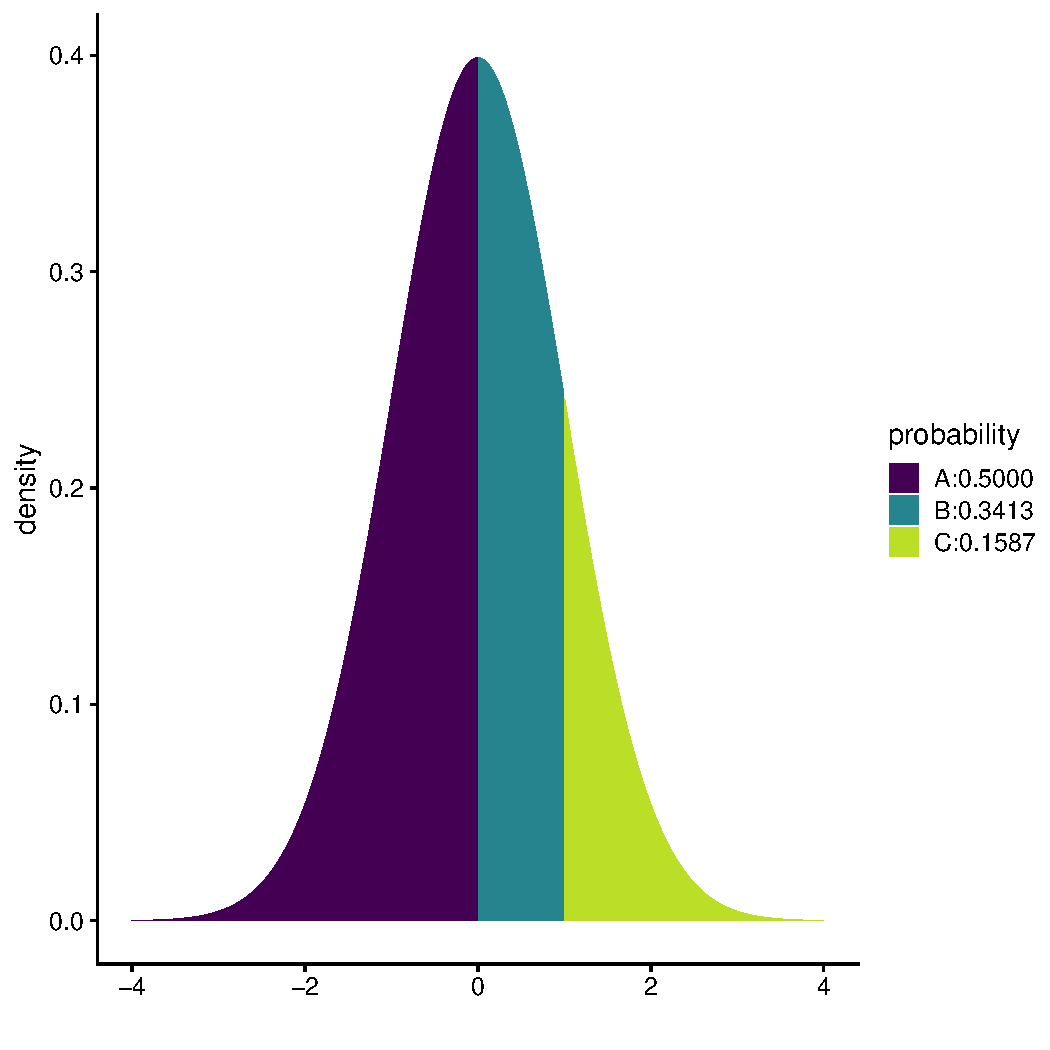
\includegraphics[width=0.60\linewidth]{figure/unnamed-chunk-1-1} 

}


\begin{kframe}\begin{verbatim}
## [1] 0.5000000 0.8413447
\end{verbatim}
\end{kframe}
\end{knitrout}
\end{frame}


\begin{frame}[fragile]{$P(0 \leq Z \leq 0.1)$}

	
\begin{knitrout}\tiny
\definecolor{shadecolor}{rgb}{0.969, 0.969, 0.969}\color{fgcolor}\begin{kframe}
\begin{alltt}
\hlstd{mosaic}\hlopt{::}\hlkwd{xpnorm}\hlstd{(}\hlkwd{c}\hlstd{(}\hlnum{0}\hlstd{,}\hlnum{1}\hlopt{/}\hlnum{10}\hlstd{))}
\end{alltt}
\end{kframe}

{\centering 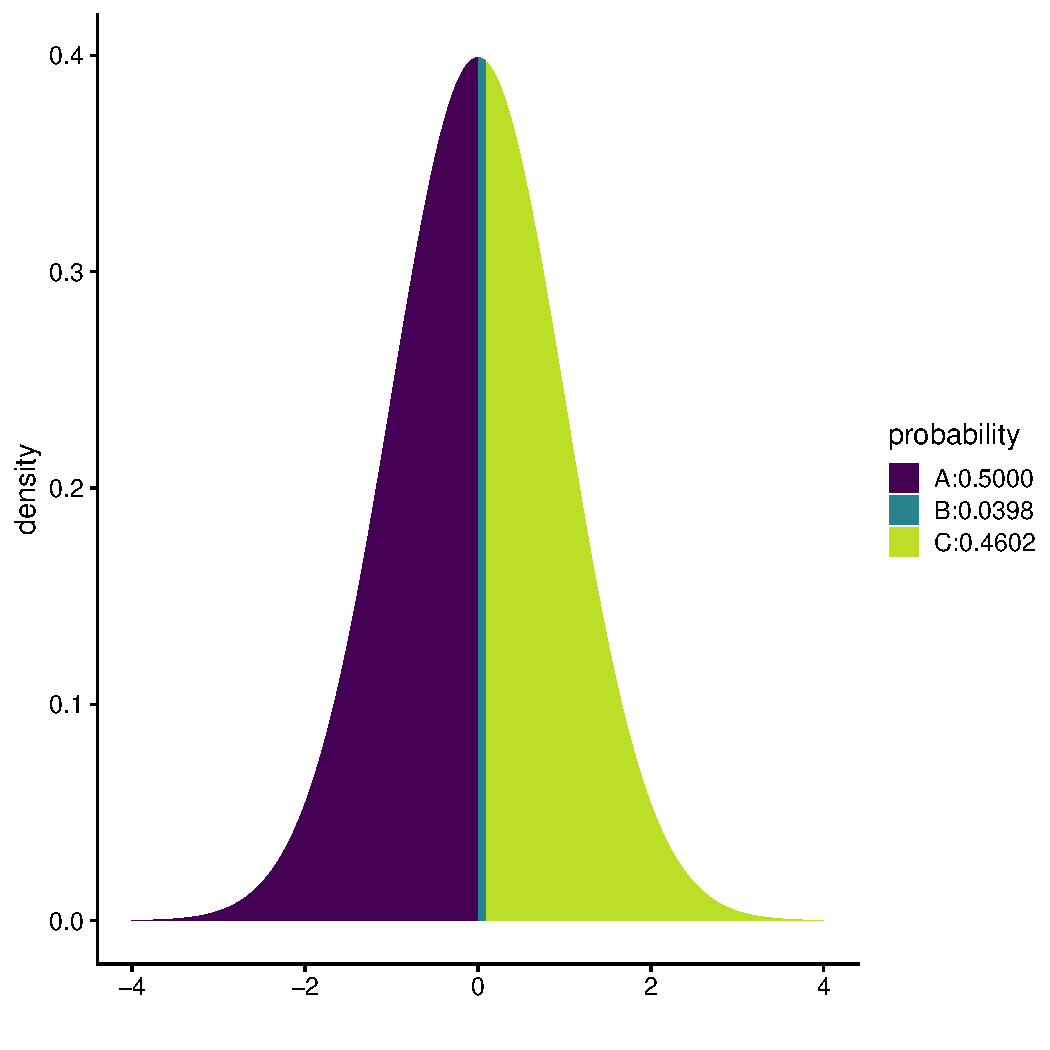
\includegraphics[width=0.60\linewidth]{figure/unnamed-chunk-2-1} 

}


\begin{kframe}\begin{verbatim}
## [1] 0.5000000 0.5398278
\end{verbatim}
\end{kframe}
\end{knitrout}
\end{frame}



\begin{frame}[fragile]{$P(0 \leq Z \leq 0.01)$}

	
\begin{knitrout}\tiny
\definecolor{shadecolor}{rgb}{0.969, 0.969, 0.969}\color{fgcolor}\begin{kframe}
\begin{alltt}
\hlstd{mosaic}\hlopt{::}\hlkwd{xpnorm}\hlstd{(}\hlkwd{c}\hlstd{(}\hlnum{0}\hlstd{,}\hlnum{1}\hlopt{/}\hlnum{100}\hlstd{))}
\end{alltt}
\end{kframe}

{\centering 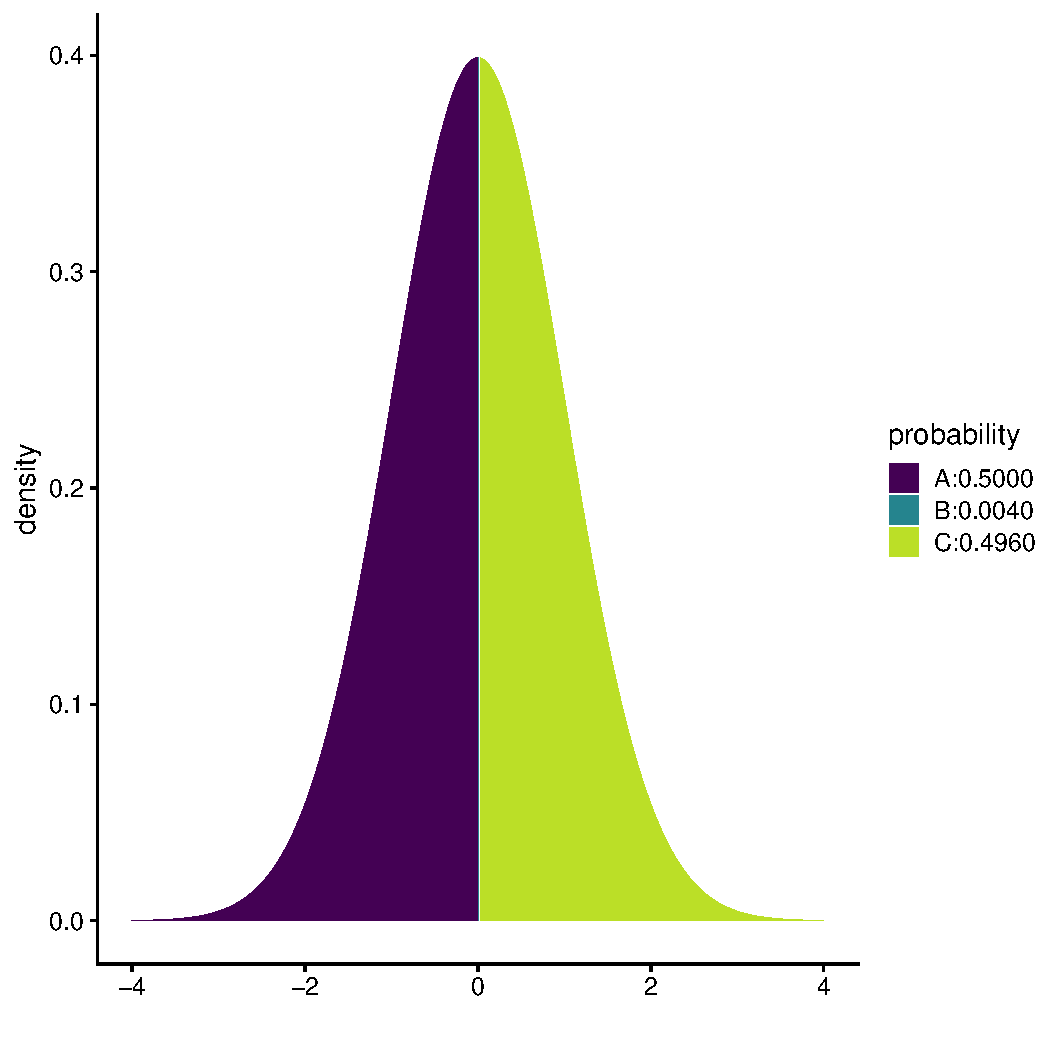
\includegraphics[width=0.60\linewidth]{figure/unnamed-chunk-3-1} 

}


\begin{kframe}\begin{verbatim}
## [1] 0.5000000 0.5039894
\end{verbatim}
\end{kframe}
\end{knitrout}
\end{frame}



\begin{frame}{How Can Every Value Have Probability 0?}
	
	\begin{itemize}
		  \setlength{\itemsep}{10pt}
		
		\item So, what’s the probability that $Z$ is exactly 0? Well, there's no
		area under the curve right at $x = 0$, so the probability is 0.
		
		\item It's only \textbf{intervals} that have positive probability, but that's OK.
		
		\item In real life we never mean exactly 0.0000000000 or any other
		value. If you say ``exactly 164 pounds,'' you might really mean
		between 163.5 and 164.5 pounds or even between 163.99
		and 164.01 pounds, but realistically not 164.000000000 . . .
		pounds
	\end{itemize}
	
\end{frame}


\section{Expected Value of a function of a RV}

\begin{frame}{Expected value for a discrete RV}
	
	\begin{definition}
		Let $Y$ be a discrete random variable with set of possible values $D=\left\lbrace y_1, y_2, \ldots,y_k  \right\rbrace$ and corresponding probabilities for each value, e.g., $y_1$ with probability $\Prob(y_1)$, $y_2$ with probability $\Prob(y_2)$, $y_3$ with probability $\Prob(y_3)$, $\ldots$, $y_k$ with probability $\Prob(y_k)$. Furthermore, let $g(Y)$ be some real-valued function of $Y$. Then the expected value of $g(Y)$ is:
		
		$$\operatorname{E}(g(Y)) =  \sum_{y \in D} g(y) \times \operatorname{P}(y)\;.$$
		i.e. it is a weighted mean of the $g(y)$'s, with $\Prob(y)$'s as weights.
	\end{definition}
	\pause 
	Let $c$ be a constant and $Z$ another random variable
	\begin{itemize}
%		\setlength{\itemsep}{10pt}		
		\item $g(Y) = Y + c$ $\rightarrow$ \pause 
		\item $g(Y) = cY$ $\rightarrow$ \pause
		\item $g(Y,Z) = Y + Z$ $\rightarrow$ 
	\end{itemize}
	
\end{frame}



\begin{frame}{Exercise: $\Expec(g(Y)) = g(E(Y))$ ?}
	
\begin{itemize}[<+->]
\setlength{\itemsep}{10pt}		
\item $Y$ = Noon Temperature (C) in Montreal on a randomly selected day of the year;  
$g(Y)$ = Temperature (F) = 32 + (9/5) $Y$
\item  $Y_1$ and $Y_2$ are two random variables that might or might not be related; $g(Y_1, Y_2) = Y_1 + Y_2$ 
\item  $g(Y_1, Y_2) = \frac{Y_1 + Y_2}{2}$  
\item $g(Y_i) = \frac{1}{n} \sum_{i=1}^{n} Y_i$
\item  $Y$ = diameter of a randomly chosen sphere; $g(Y)$ = Volume of sphere = $\frac{\pi}{6}  Y^3$
\end{itemize}
	
\end{frame}


\begin{frame}{Example: $g(Y)$ = Volume of sphere = $\frac{\pi}{6}  Y^3$}

\end{frame}

\begin{frame}[fragile]{Example: Checking via simulation}
\begin{columns}
		\begin{column}{0.5\textwidth}  %%<--- here
\begin{knitrout}\tiny
\definecolor{shadecolor}{rgb}{0.969, 0.969, 0.969}\color{fgcolor}\begin{kframe}
\begin{alltt}
\hlstd{g.y} \hlkwb{<-} \hlkwa{function}\hlstd{(}\hlkwc{y}\hlstd{) \{}
 \hlstd{(pi} \hlopt{/} \hlnum{6}\hlstd{)} \hlopt{*} \hlstd{y}\hlopt{^}\hlnum{3}
\hlstd{\}}

\hlkwd{set.seed}\hlstd{(}\hlnum{12}\hlstd{)}
\hlstd{B} \hlkwb{<-} \hlnum{1000}\hlstd{; N} \hlkwb{<-} \hlnum{2000}
\hlstd{E_g.y} \hlkwb{<-} \hlkwd{replicate}\hlstd{(B, \{}
  \hlstd{diameter} \hlkwb{<-} \hlkwd{runif}\hlstd{(N,} \hlkwc{min} \hlstd{=} \hlnum{0}\hlstd{,} \hlkwc{max} \hlstd{=} \hlnum{10}\hlstd{)}
  \hlkwd{mean}\hlstd{(}\hlkwd{g.y}\hlstd{(diameter))} \hlcom{# E(g(y))}
\hlstd{\})}

\hlstd{g_E.y} \hlkwb{<-} \hlkwd{replicate}\hlstd{(B, \{}
  \hlstd{diameter} \hlkwb{<-} \hlkwd{runif}\hlstd{(N,} \hlkwc{min} \hlstd{=} \hlnum{0}\hlstd{,} \hlkwc{max} \hlstd{=} \hlnum{10}\hlstd{)}
  \hlkwd{g.y}\hlstd{(}\hlkwd{mean}\hlstd{(diameter))} \hlcom{# g(E(y))}
\hlstd{\})}

\hlkwd{par}\hlstd{(}\hlkwc{mfrow} \hlstd{=} \hlkwd{c}\hlstd{(}\hlnum{1}\hlstd{,}\hlnum{2}\hlstd{))}
\hlkwd{hist}\hlstd{(E_g.y,} \hlkwc{col} \hlstd{=} \hlstr{"lightblue"}\hlstd{,} \hlkwc{xlab} \hlstd{=} \hlstr{"mean(g(y))"}\hlstd{,}
     \hlkwc{main} \hlstd{=} \hlkwd{sprintf}\hlstd{(}\hlstr{"Average of E(g(Y)) over 1000\textbackslash{}n replications 
     is %0.2f"}\hlstd{,}\hlkwd{mean}\hlstd{(E_g.y)))}
\hlkwd{abline}\hlstd{(}\hlkwc{v} \hlstd{=} \hlkwd{mean}\hlstd{(E_g.y),} \hlkwc{col} \hlstd{=} \hlstr{"red"}\hlstd{,} \hlkwc{lty} \hlstd{=} \hlnum{2}\hlstd{,} \hlkwc{lwd} \hlstd{=} \hlnum{3}\hlstd{)}

\hlkwd{hist}\hlstd{(g_E.y,} \hlkwc{col} \hlstd{=} \hlstr{"lightblue"}\hlstd{,} \hlkwc{xlab} \hlstd{=} \hlstr{"g(mean(y))"}\hlstd{,}
     \hlkwc{main} \hlstd{=} \hlkwd{sprintf}\hlstd{(}\hlstr{"Average of g(E(Y)) over 1000\textbackslash{}n replications 
     is %0.2f"}\hlstd{,}\hlkwd{mean}\hlstd{(g_E.y)))}
\hlkwd{abline}\hlstd{(}\hlkwc{v} \hlstd{=} \hlkwd{mean}\hlstd{(g_E.y),} \hlkwc{col} \hlstd{=} \hlstr{"red"}\hlstd{,} \hlkwc{lty} \hlstd{=} \hlnum{2}\hlstd{,} \hlkwc{lwd} \hlstd{=} \hlnum{3}\hlstd{)}
\end{alltt}
\end{kframe}
\end{knitrout}
\end{column}
		\begin{column}{0.5\textwidth}  %%<--- here
\begin{knitrout}\tiny
\definecolor{shadecolor}{rgb}{0.969, 0.969, 0.969}\color{fgcolor}

{\centering 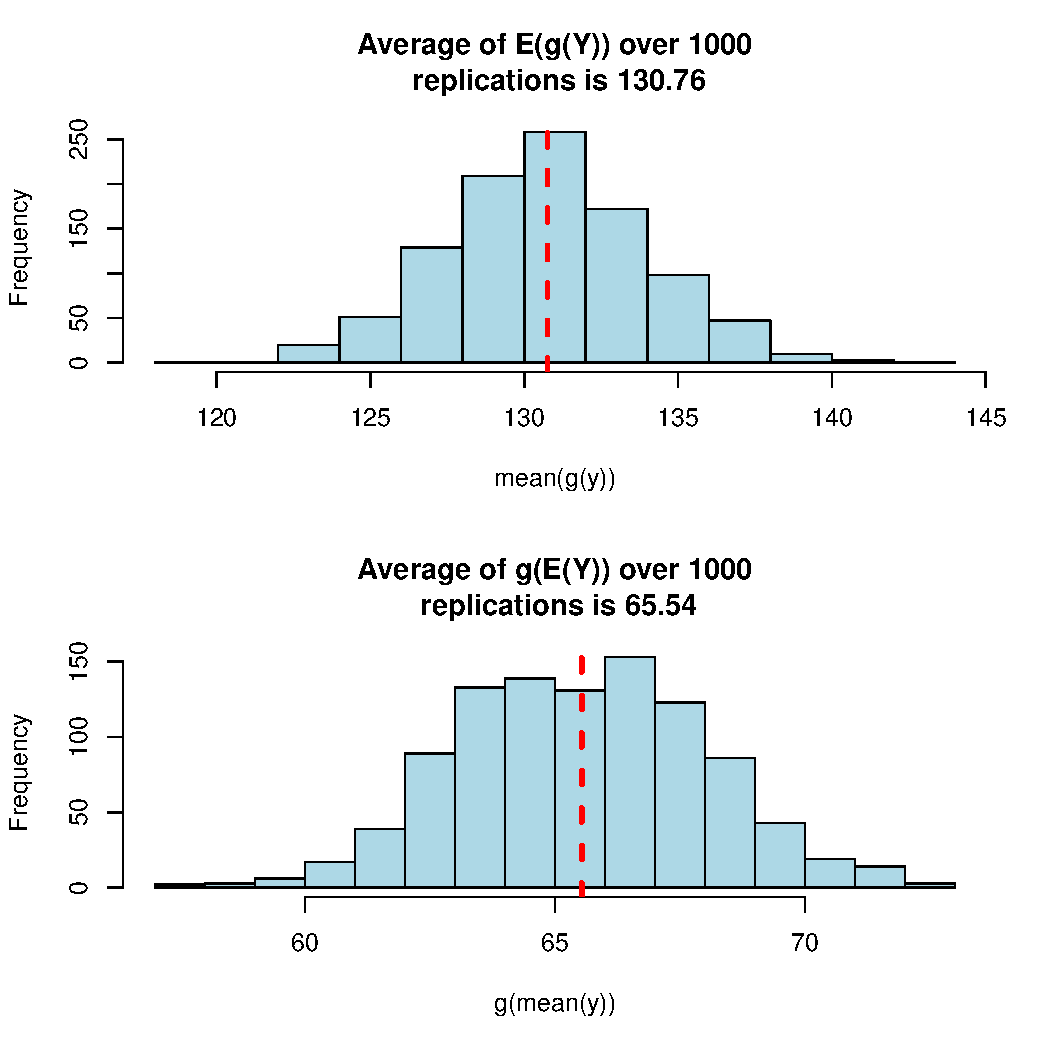
\includegraphics[width=\maxwidth]{figure/unnamed-chunk-5-1} 

}


\end{knitrout}
\end{column}
\end{columns}
\end{frame}


\begin{frame}[fragile]{Example: Checking the results theoretically}
	\begin{itemize}
		\item We \href{https://en.wikipedia.org/wiki/Continuous_uniform_distribution#Moments}{know} for $Y \sim Uniform(a, b)$, the n$^{th}$ moment $\Expec(Y^n)$ is given by:
		$$
		\Expec(Y^n) = \frac{b^{n+1} - a^{n+1}}{(n+1)(b-a)}
		$$
		\pause
		\item Therefore, we know, theoretically, for $Y \sim Uniform(0, 10)$: 
		
		\begin{align}
		\Expec(Y) &= \textcolor{white}{tsgkldsgkldhgkdshkgextknglkdsngksdnglknsd} \\
		\Expec(Y^3) &= \textcolor{white}{tsgkldsgkldhgkdshkgextknglkdsngksdnglknsd}
		\end{align}
		\pause		
		\item It follows that, theoretically, 
		\begin{align}
			\Expec(g(Y)) & = 130.9\\
			g(\Expec(Y)) & = 65.45
		\end{align}
	\end{itemize}
\end{frame}





\section{Variance and SD of a function of a RV}

\begin{frame}{Variance of an RV}
	\begin{definition}
The variance of the random variable $Y$ is given by $$\Var(Y) = \Expec[(Y - \mu)^2].$$ 
\begin{itemize}
	\item Discrete RV: $\Var(Y) = \sum_y (y - \Expec(Y))^2 \times f(y)$
	\item Continous RV: $\Var(Y) = \int_y (y - \Expec(Y))^2 \times f(y) \partial y$
\end{itemize}
	\end{definition}


\end{frame}

\begin{frame}[fragile]{Graphical representation of variance of a RV}
\begin{knitrout}\tiny
\definecolor{shadecolor}{rgb}{0.969, 0.969, 0.969}\color{fgcolor}

{\centering 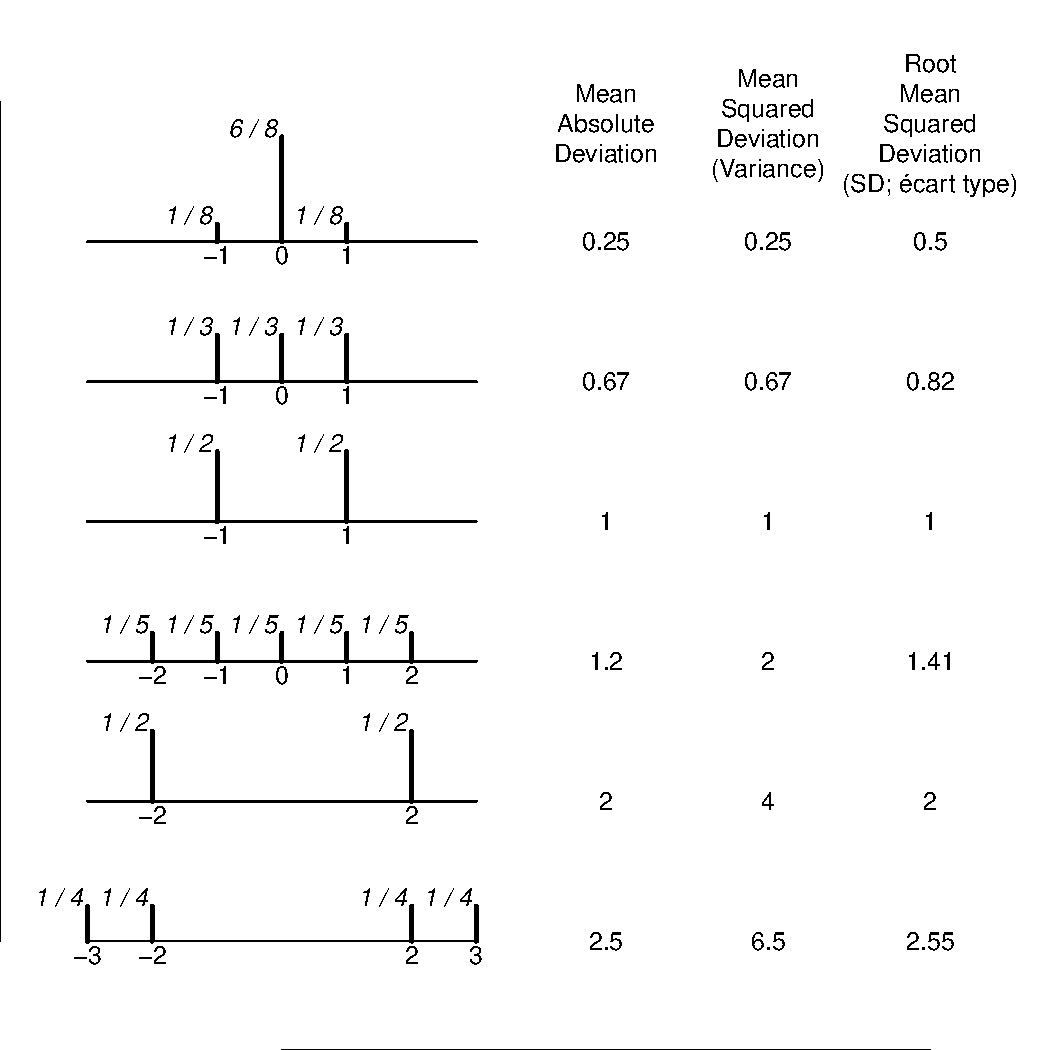
\includegraphics[width=0.85\linewidth]{figure/unnamed-chunk-6-1} 

}


\end{knitrout}
	
\end{frame}



\begin{frame}{Variance of a function of a RV}
	
\begin{itemize}
\setlength{\itemsep}{20pt}		
\item $Y$ = Noon Temperature (C) in Mtl on a randomly selected day of the year;  $g(Y)$ = Temperature (F) = 32 + (9/5) $Y$ \pause
\item $Y$ = Years of publication of all the books in the McGill Library, with Years measured from 1439 AD;  $W = Y - 1439$ vs. $W = 2020 - Y$
\end{itemize}	

\end{frame}




\section{Sums, means, differences of random variables}

\begin{frame}[fragile]{A sum of 2 random variables}
	

	
	
	
		\begin{columns}
		\begin{column}{0.5\textwidth}  %%<--- here
\begin{knitrout}\tiny
\definecolor{shadecolor}{rgb}{0.969, 0.969, 0.969}\color{fgcolor}

{\centering 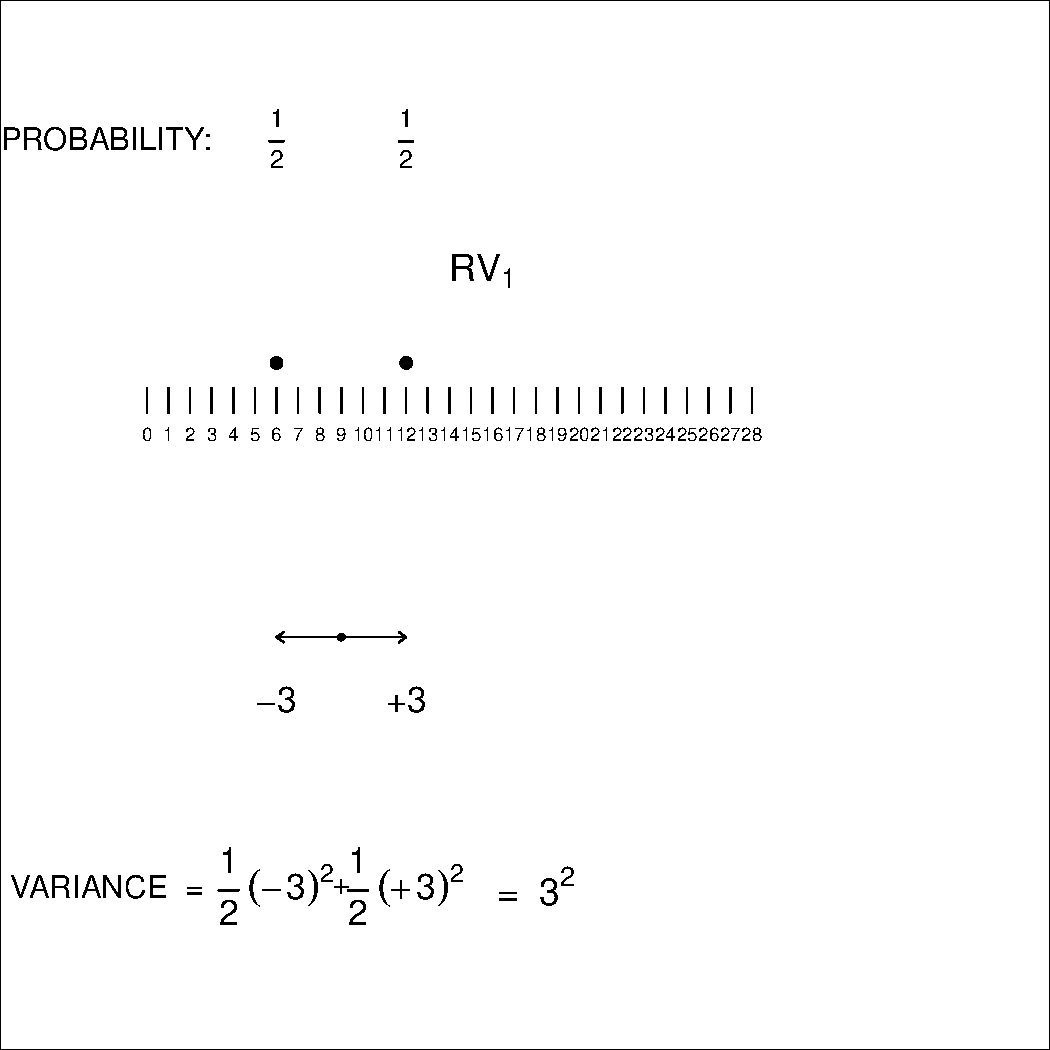
\includegraphics[width=1\linewidth]{figure/unnamed-chunk-8-1} 

}


\end{knitrout}
			
					\end{column}
		\begin{column}{0.5\textwidth}
\begin{knitrout}\tiny
\definecolor{shadecolor}{rgb}{0.969, 0.969, 0.969}\color{fgcolor}

{\centering 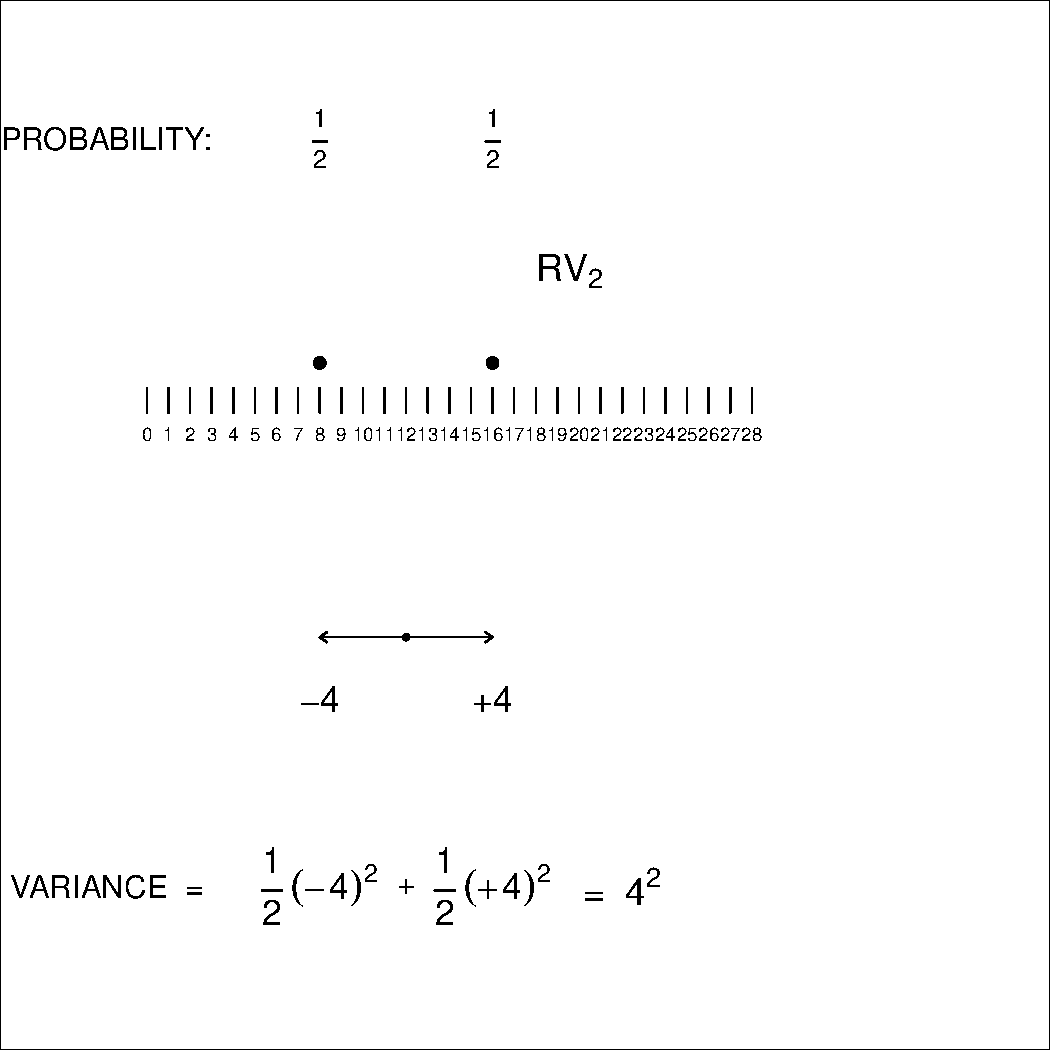
\includegraphics[width=1\linewidth]{figure/unnamed-chunk-9-1} 

}


\end{knitrout}
	\end{column}
	\end{columns}
	
\end{frame}

\begin{frame}[fragile,plain]
\begin{knitrout}\tiny
\definecolor{shadecolor}{rgb}{0.969, 0.969, 0.969}\color{fgcolor}

{\centering 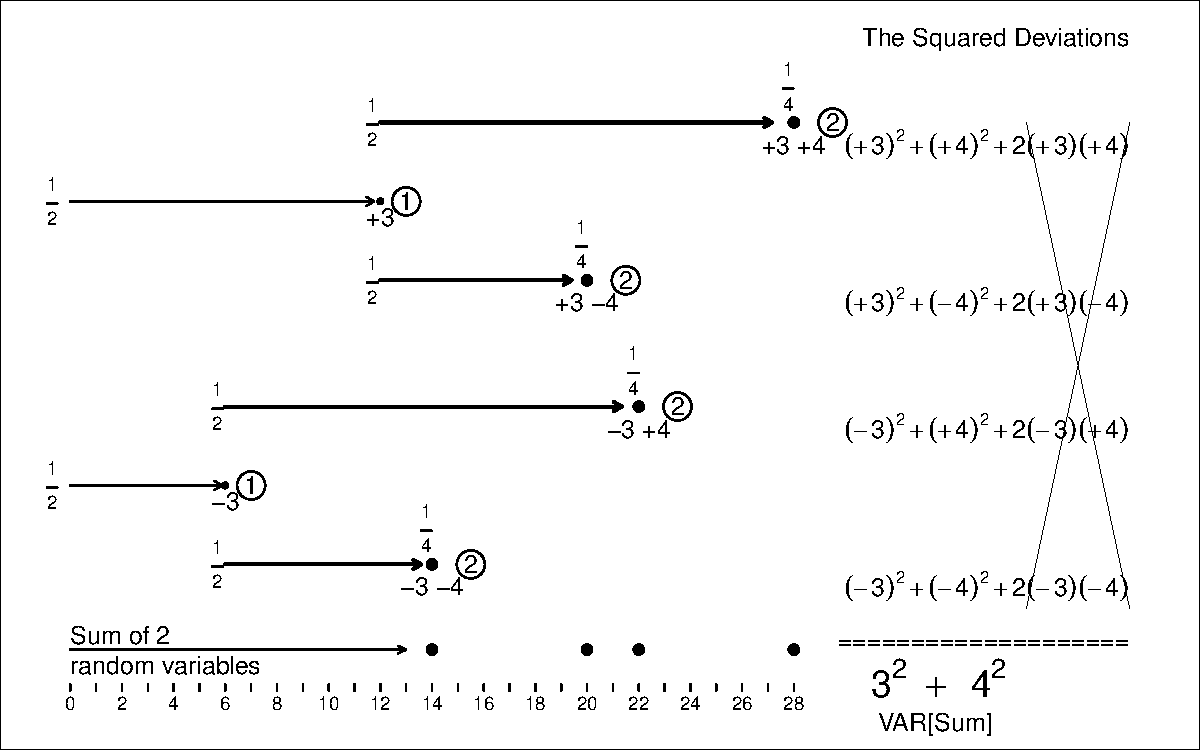
\includegraphics[width=\maxwidth]{figure/unnamed-chunk-10-1} 

}


\end{knitrout}

\end{frame}




\begin{frame}[fragile]{Application: Measurement errors}
	
\begin{knitrout}\tiny
\definecolor{shadecolor}{rgb}{0.969, 0.969, 0.969}\color{fgcolor}

{\centering 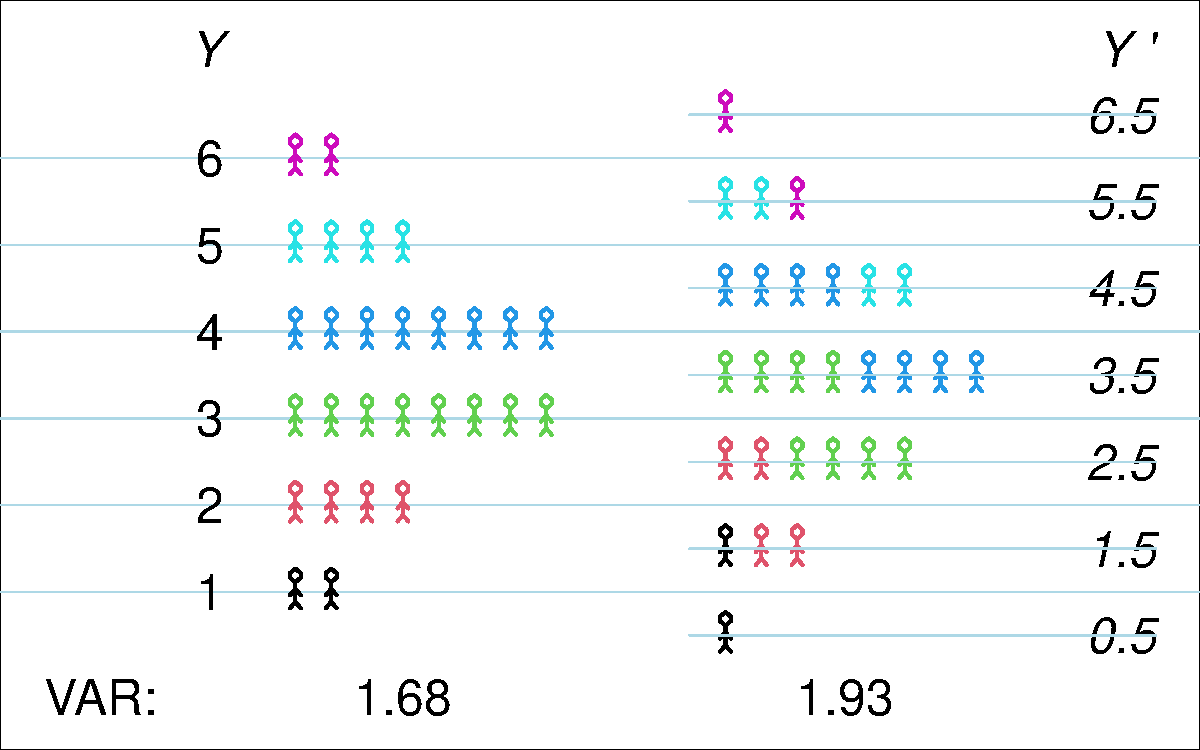
\includegraphics[width=\maxwidth]{figure/unnamed-chunk-11-1} 

}


\end{knitrout}
	
\end{frame}


\begin{frame}[fragile]{A sum of $n$ random variables}
	
	\begin{itemize}
		\setlength{\itemsep}{10pt}		
	\item Up to now, to keep things general, we used $n$ non-identical -- but independent -- random variables. If we
	consider the Variance and the sum of $n$ \textbf{identical} -- and independent -- random variables, so the $n$ Variances (each abbreviated to $\Var$) are all equal, the laws simplify:
	
	\item First, since the variances add, we have that	
	$$ \Var(RV_1 + RV_2 + \dots + RV_n) = \Var_1 + \Var_2 + \dots + \Var_n = n \times \ each \ \Var.$$
	
\item Taking square roots,	
	$$ SD( \ RV_1 + RV_2 + \dots + RV_n \ ) = \sqrt{ \ n \times \ \textrm{each} \ \Var} = \sqrt{n} \ \times \ \textrm{each} \ SD$$
	
	\pause

	\item $$ SD\bigg(\frac{RV_1 + RV_2 + \dots + RV_n}{n}\bigg) = \frac{\sqrt{n} \ \times \ \textrm{each} \ SD}{n} = \frac{\textrm{common} \ SD}{\sqrt{n}} $$
	
	\item $$ \Var\bigg(\frac{RV_1 + RV_2 + \dots + RV_n}{n}\bigg) = \frac{\textrm{common} \ \Var}{n} $$
	

		 
\end{itemize}

\end{frame}


\begin{frame}[fragile]{Example: Length of Words in a Book - $n = 1$ word}
\begin{knitrout}\tiny
\definecolor{shadecolor}{rgb}{0.969, 0.969, 0.969}\color{fgcolor}

{\centering 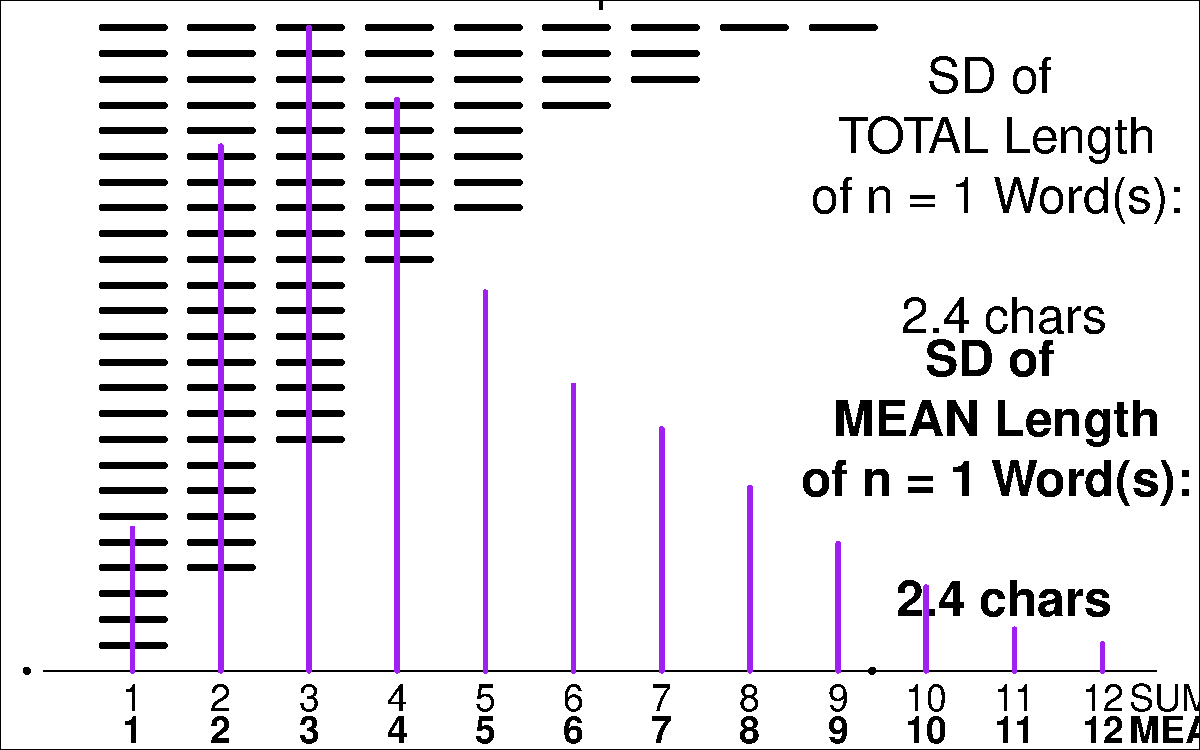
\includegraphics[width=\maxwidth]{figure/unnamed-chunk-12-1} 

}


\end{knitrout}
\end{frame}

\begin{frame}[fragile]{$n = 4$ words}
\begin{knitrout}\tiny
\definecolor{shadecolor}{rgb}{0.969, 0.969, 0.969}\color{fgcolor}

{\centering 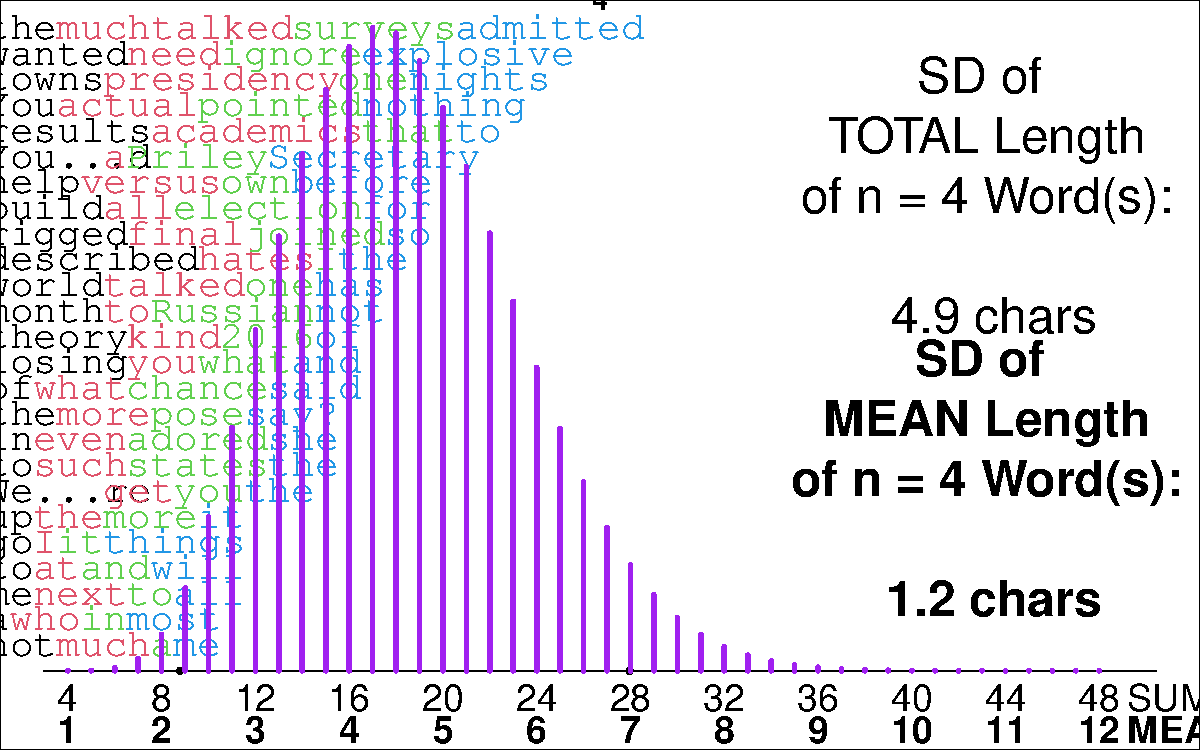
\includegraphics[width=\maxwidth]{figure/unnamed-chunk-13-1} 

}


\end{knitrout}
\end{frame}


\begin{frame}[fragile]{$n = 9$ words}
\begin{knitrout}\tiny
\definecolor{shadecolor}{rgb}{0.969, 0.969, 0.969}\color{fgcolor}

{\centering 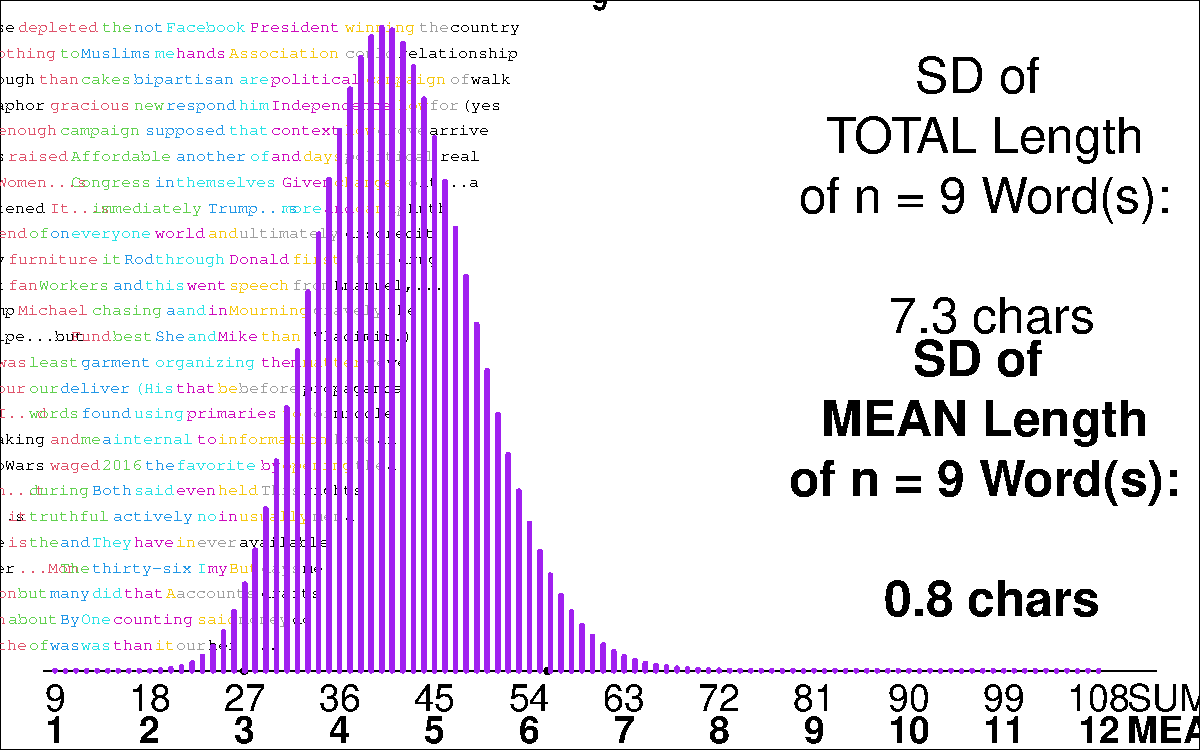
\includegraphics[width=\maxwidth]{figure/unnamed-chunk-14-1} 

}


\end{knitrout}
\end{frame}



\begin{frame}[fragile]{Difference of 2 Random Variables via Simulation}
\begin{knitrout}\tiny
\definecolor{shadecolor}{rgb}{0.969, 0.969, 0.969}\color{fgcolor}\begin{kframe}
\begin{alltt}
\hlkwd{set.seed}\hlstd{(}\hlnum{12}\hlstd{)}
\hlstd{B} \hlkwb{<-} \hlnum{999}\hlstd{; N} \hlkwb{<-} \hlnum{200}
  \hlstd{var_diff} \hlkwb{<-} \hlkwd{replicate}\hlstd{(B, \{}
  \hlstd{RV1} \hlkwb{<-} \hlkwd{rnorm}\hlstd{(N,} \hlkwc{mean} \hlstd{=} \hlnum{2}\hlstd{,} \hlkwc{sd} \hlstd{=} \hlnum{3}\hlstd{)}
  \hlstd{RV2} \hlkwb{<-} \hlkwd{rnorm}\hlstd{(N,} \hlkwc{mean} \hlstd{=} \hlnum{4}\hlstd{,} \hlkwc{sd} \hlstd{=} \hlnum{4}\hlstd{)}
  \hlkwd{var}\hlstd{(RV1} \hlopt{-} \hlstd{RV2)}
\hlstd{\})}

\hlkwd{hist}\hlstd{(var_diff,} \hlkwc{col} \hlstd{=} \hlstr{"lightblue"}\hlstd{,} \hlkwc{xlab} \hlstd{=} \hlstr{"Var(RV1 - RV2)"}\hlstd{,}
    \hlkwc{main} \hlstd{=} \hlkwd{sprintf}\hlstd{(}\hlstr{"Median of Var(RV1-RV2) over 999 replications is %0.2f"}\hlstd{,}\hlkwd{median}\hlstd{(var_diff)))}
\hlkwd{abline}\hlstd{(}\hlkwc{v} \hlstd{=} \hlkwd{median}\hlstd{(var_diff),} \hlkwc{col} \hlstd{=} \hlstr{"red"}\hlstd{,} \hlkwc{lty} \hlstd{=} \hlnum{2}\hlstd{,} \hlkwc{lwd} \hlstd{=} \hlnum{3}\hlstd{)}
\end{alltt}
\end{kframe}

{\centering 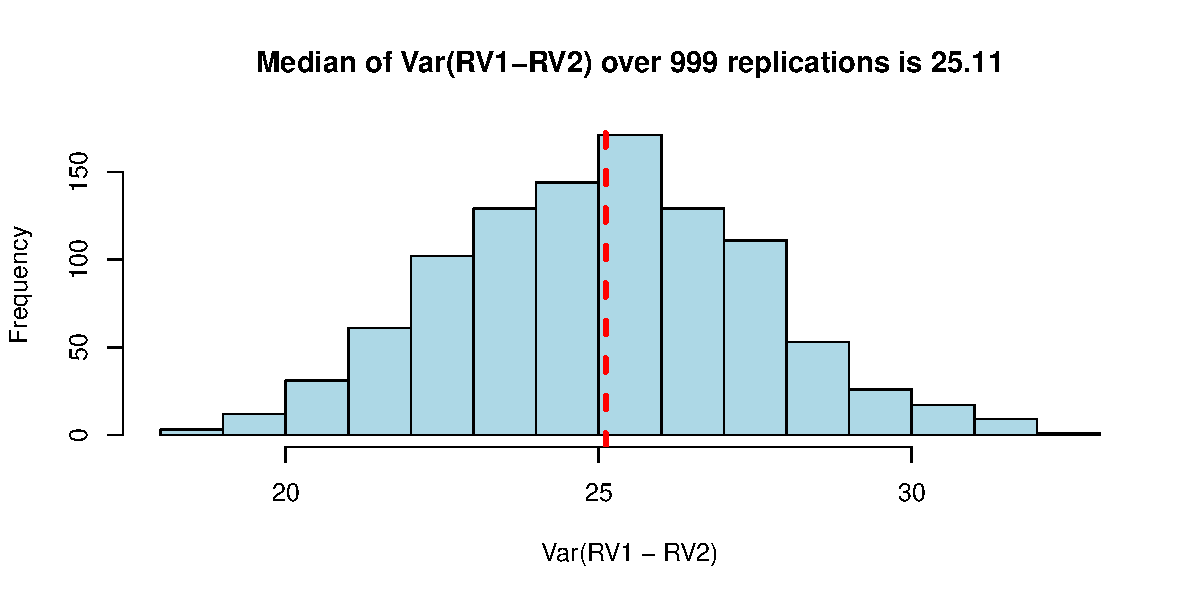
\includegraphics[width=\maxwidth]{figure/unnamed-chunk-15-1} 

}


\end{knitrout}
\end{frame}



\section{Linear combinations of random variables (regression slopes)}


\begin{frame}[fragile]{Linear Combinations of random variables}
\begin{knitrout}\tiny
\definecolor{shadecolor}{rgb}{0.969, 0.969, 0.969}\color{fgcolor}

{\centering 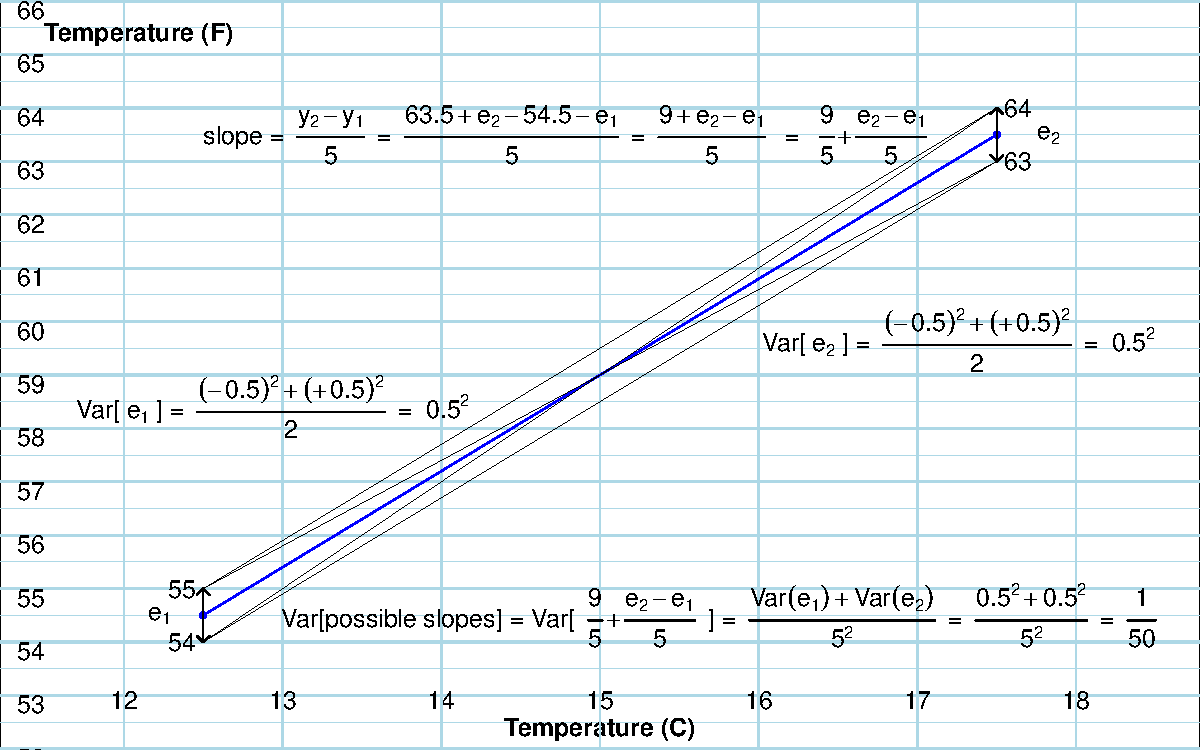
\includegraphics[width=\maxwidth]{figure/unnamed-chunk-16-1} 

}


\end{knitrout}

\end{frame}






	\begin{frame}[fragile]{Session Info}
	\tiny
	
\begin{knitrout}\tiny
\definecolor{shadecolor}{rgb}{0.969, 0.969, 0.969}\color{fgcolor}\begin{kframe}
\begin{verbatim}
R version 4.0.4 (2021-02-15)
Platform: x86_64-pc-linux-gnu (64-bit)
Running under: Pop!_OS 21.04

Matrix products: default
BLAS:   /usr/lib/x86_64-linux-gnu/openblas-pthread/libblas.so.3
LAPACK: /usr/lib/x86_64-linux-gnu/openblas-pthread/libopenblasp-r0.3.13.so

attached base packages:
[1] tools     stats     graphics  grDevices utils     datasets  methods  
[8] base     

other attached packages:
 [1] DT_0.16           mosaic_1.7.0      Matrix_1.3-2      mosaicData_0.20.1
 [5] ggformula_0.9.4   ggstance_0.3.4    lattice_0.20-41   kableExtra_1.2.1 
 [9] socviz_1.2        gapminder_0.3.0   here_0.1          NCStats_0.4.7    
[13] FSA_0.8.30        forcats_0.5.1     stringr_1.4.0     dplyr_1.0.7      
[17] purrr_0.3.4       readr_1.4.0       tidyr_1.1.3       tibble_3.1.3     
[21] ggplot2_3.3.5     tidyverse_1.3.0   knitr_1.33       

loaded via a namespace (and not attached):
 [1] fs_1.5.0           lubridate_1.7.9    webshot_0.5.2      httr_1.4.2        
 [5] rprojroot_2.0.2    backports_1.2.1    utf8_1.2.2         R6_2.5.1          
 [9] DBI_1.1.1          colorspace_2.0-2   withr_2.4.2        tidyselect_1.1.1  
[13] gridExtra_2.3      leaflet_2.0.3      curl_4.3.2         compiler_4.0.4    
[17] cli_3.0.1          rvest_1.0.0        pacman_0.5.1       xml2_1.3.2        
[21] ggdendro_0.1.22    labeling_0.4.2     mosaicCore_0.8.0   scales_1.1.1      
[25] digest_0.6.27      foreign_0.8-81     rmarkdown_2.9.7    rio_0.5.16        
[29] pkgconfig_2.0.3    htmltools_0.5.2    highr_0.9          dbplyr_1.4.4      
[33] fastmap_1.1.0      htmlwidgets_1.5.3  rlang_0.4.11       readxl_1.3.1      
[37] rstudioapi_0.13    farver_2.1.0       generics_0.1.0     jsonlite_1.7.2    
[41] crosstalk_1.1.1    zip_2.2.0          car_3.0-9          magrittr_2.0.1    
[45] Rcpp_1.0.7         munsell_0.5.0      fansi_0.5.0        abind_1.4-5       
[49] lifecycle_1.0.0    stringi_1.7.3      carData_3.0-4      MASS_7.3-53.1     
[53] plyr_1.8.6         grid_4.0.4         blob_1.2.1         ggrepel_0.8.2     
[57] crayon_1.4.1       cowplot_1.1.0      haven_2.3.1        splines_4.0.4     
[61] hms_1.0.0          pillar_1.6.2       reprex_0.3.0       glue_1.4.2        
[65] evaluate_0.14      data.table_1.14.0  modelr_0.1.8       vctrs_0.3.8       
[69] tweenr_1.0.1       cellranger_1.1.0   gtable_0.3.0       polyclip_1.10-0   
[73] assertthat_0.2.1   TeachingDemos_2.12 xfun_0.25          ggforce_0.3.2     
[77] openxlsx_4.1.5     broom_0.7.2        viridisLite_0.4.0  ellipsis_0.3.2    
\end{verbatim}
\end{kframe}
\end{knitrout}
	
\end{frame}


\end{document}


